\newpage
\chapter{Additional Neural IR models studied}

This chapter presents more neural models that were compared to
DRMM. It was an opportunity for me to explore different approaches;
moreover I created some drafts implementation of them all, but due
to time constraints I haven't been able to properly test them.

\section{Deep Structured Semantic Model}
\label{sec:dssm}

The Deep Structured Semantic Model (DSSM, \cite{dssm}) is one
architecture based on the Siamese network that trains on query and document
title pairs where both the pieces of texts are represented as
bags-of-character trigraphs.

The advantage of character trigraphs is mainly the dictionary size reduction
(the authors observed on their real-word dataset a reduction from 500K word in vocabulary to 300K).

The DSSM architecture consists of two deep models (for the query and the
document) with all fully-connected layers and cosine distance as the choice of
similarity function in the middle.

Huang et al. proposed to train the model on clickthrough data where
each training sample consists of a query Q, and a set $\mathcal{D}$ of positive
documents (documents clicked by a user on the SERP for that query - $d^+$) plus
k=4 randomly selected negative documents for each positive one.

\begin{figure}[H]
  \centering
  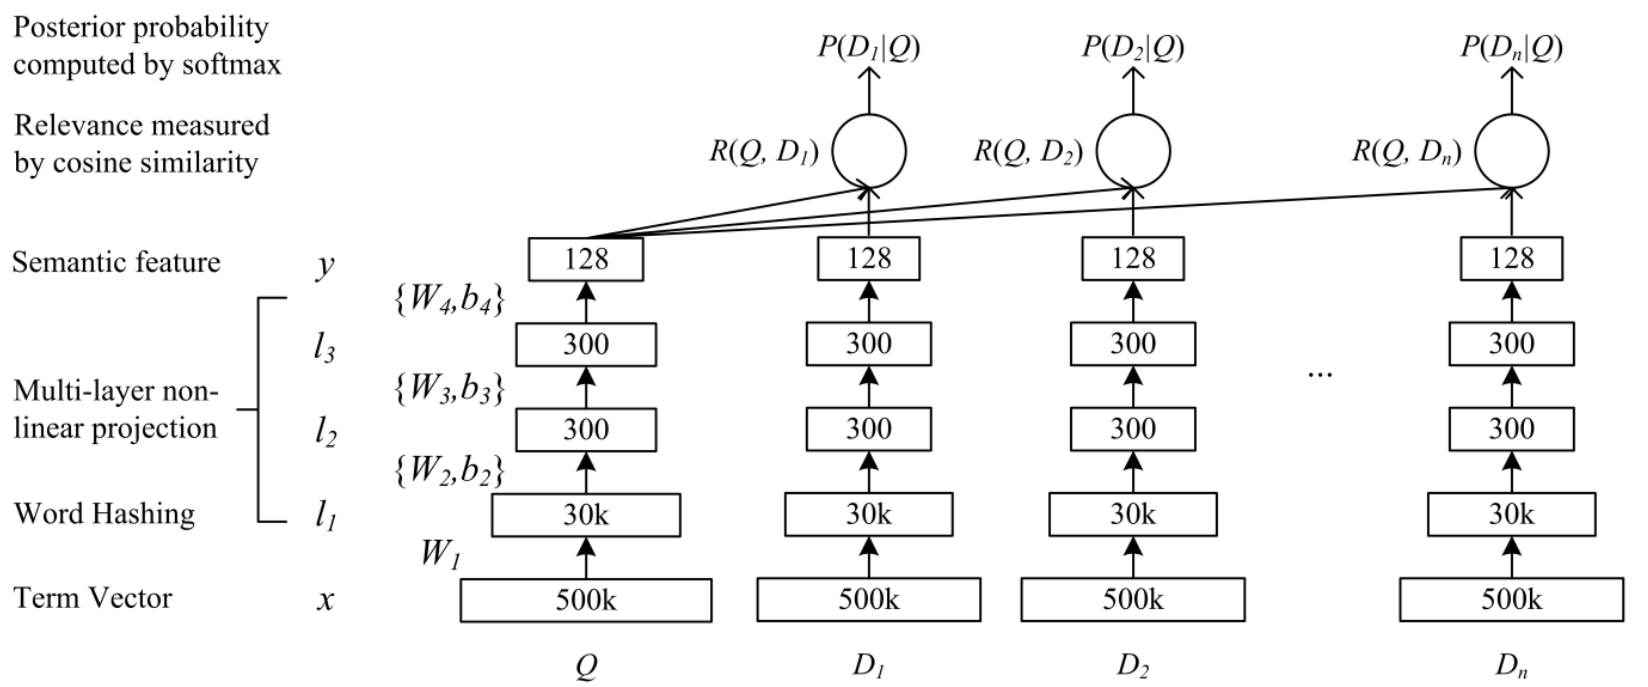
\includegraphics[width=0.9\textwidth]{DSSM.png}
  \caption{DSSM architecture}
  \label{fig:dssm_arch}
\end{figure}

Let $\vec{x}$ be the input term vector, $\vec{y}$ the output vector,
$l_i \quad i = 1...N-1$ the intermediate hidden layers, $W_i$ the i-th weight
matrix, and $b_i$ the i-th bias term, we have:

\begin{equation}
\tag{Input to first layer}
l_1 = W_1 x
\end{equation}

\begin{equation}
\tag{input to i-th layer}
l_i = tanh(W_i l_{i-1} + b_i), i = 2...N-1
\end{equation}

\begin{equation}
\tag{output layer}
y = tanh(W_N l_{N-1} + b_N)
\end{equation}

where we use \textbf{tahn} as the activation function at the output layer and
the hidden layers $l_i, i = 1...N-1$.

The semantic relevance score between a query and a document is then measured
as the cosine similarity of the respective output from final layer $R(Q, d) = R(y^{(Q)}, y^{(d)})$ (see equation \ref{eq:cosine}).

The model is trained to maximize the likelihood of the clicked documents given
the queries across the training set.

\begin{equation}
\mathcal{L}_{dssm} (Q, d^+) = -log (\prod_{Q,d^+} P(d^+|Q))
\end{equation}

where P(d|Q) is:

\begin{equation}
P(d|Q) = \frac{e^{\gamma R(Q, d)}}{\sum_{d' \in \mathcal{D}} \gamma R(Q, d')}
\end{equation}

\section{Convolutional Deep Structured Semantic Model}

This is a latent semantic model based on a convolutional neural network and
has the purpose to learn low-dimensional semantic vectors for search queries
and web documents (\cite{cdssm}).

Most latent semantic models manipulate a query (or a document) as
a bag of words, so they aren't effective in capturing contextual structures
needed for IR.

Usually the information captured by models such as TF-IDF, BM25 and topic models
isn't often enough to be effective; thus, as a separate line of research, deep learning based techniques have been proposed for semantic understanding.

Compared with DSSM, C-DSSM still uses the same word hashing layer but has a new convolutional layer that projects each word
within a context window to a local contextual feature vector and then uses a max pooling layer to extract the most salient local features to
form a fixed-length global feature vector.

Semantically similar words-within-context are projected to vectors that are
close to each other in the contextual feature space.

The global feature vector can be then fed to feed-forward neural network layers,
which perform affine transformations followed by non-linear functions applied
element-wise over their inputs to extract highly non-linear and effective
features.

\begin{figure}[H]
  \centering
  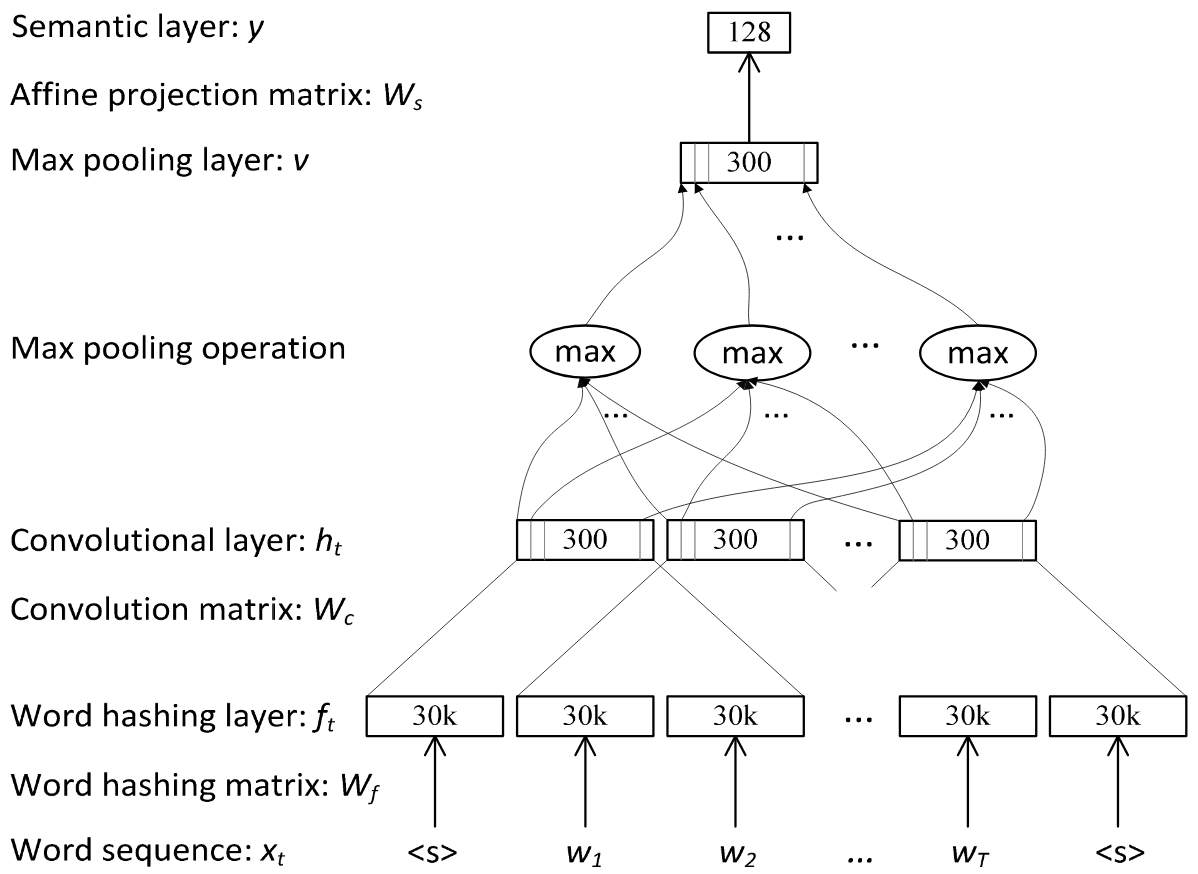
\includegraphics[width=0.9\textwidth]{cdssm_arch.png}
  \caption{CDSSM architecture}
  \label{fig:cdssm_arch}
\end{figure}

The semantic relevance score between a query and a document is then measured
as in \ref{sec:dssm} (their cosine similarity R(Q, d) (see equation
\ref{eq:cosine})).

The parameters of the C-DSSM to be learned include convolution matrix $W_c$ and
semantic projection matrix $W_s$, as  illustrated (\ref{fig:cdssm_arch}).

The C-DSSM is trained on clickthrough data by maximizing the conditional
likelihood of the clicked documents given a query, using stochastic gradient
ascent.

\section{Convolutional Neural Network Architectures for
Matching Natural Language Sentences - ARC I and ARC II}

As previously stated, semantic matching is of central importance to many natural
language tasks and can enhance ad-hoc retrieval.

Natural language sentences have complicated structures, both sequential and
hierarchical, that are essential for understanding them.

A successful sentence-matching algorithm therefore needs to capture not only
the internal structures of sentences but also the rich patterns in their
interactions.

As a step toward this goal, \cite{arc} proposed a convolutional neural network
models for matching two sentences.

The proposed model represent the hierarchical structures of
sentences with their layer by-layer composition and pooling, but also capture
the rich matching patterns at different levels.

The model doesn't requires prior knowledge on language, and can be applied to
matching tasks of different nature and in different languages.

\section{Convolutional Sentence Model}
\label{sec:arcI}

It takes as input the embeddings of words (often trained beforehand with unsupervised methods) in a sentence \textit{s} aligned sequentially, and summarize the
meaning of a sentence through layers of convolution and pooling, until reaching
a fixed length vectorial representation in the final layer.

Let $\vec{s} = [w_1, w_2, \dots w_n]$ be the input sentence. The embeddings of words are represented in input as their respective transposed vectors:
input $\vec{x} = [x_1^t, x_2^t, \dots x_n^t]$ where $x_i^t$ is the vector (embedding)
transposed of the i-th word in the sentence.

\subsection{Convolutional layer}

The convolution in the first layer operates on sliding windows of words
(width $k_1$), and the convolutions in deeper layers are defined in a
similar way.

Notation:

\begin{itemize}
\item $z_i^{l,f} (x)$ is the output of a filter of type f for location i in layer l
\item $w^{l,f}$ are the parameters (weights) of the filter with type f on layer l
\item $\sigma (.)$ is the activation function
\item $\hat{z}_i^l$ is the segment of layer l for the convolution at location i (concatenates the $k_1$ vectors in the slide - at layer 0 this corresponds to concatenate the vectors of the $k_1$ words from the input
sentence x)
\end{itemize}

The convolution unit for feature map of type f (among $F_l$ of them) on Layer-l is:

\begin{equation}
\tag{Convolution / output for a filter in ARC-I}
\label{eq:conv1}
z_i^{l,f} (x) = \sigma(w^{l,f} \cdot \hat{z}_i^{l-1} + b^{l,f}) \qquad
\forall f = 1 \cdots F_l
\end{equation}

\subsubsection{Pooling layer}

Max pooling is performed every two unit window for every filter type f \textbf{after each convolution} and takes the max value \textit{c} in each pooling window (2x2).

Pooling shrinks the size of the representation by half, thus quickly
absorbs the differences in length for sentence representation, and filters out
undesirable composition of words.

Length variability is addressed by inserting all zero padding at the end of
a sentence.

To eliminate the boundary effect caused
by the great variability of sentence lengths, \cite{arc} added to the
convolutional unit a gate g which sets the output vectors to all-zeros if the
input is all zeros ($sum(\vec{v}) = 0 \implies g(\vec{v}) = 0$)
So, the equation \ref{eq:conv1} becomes:

\begin{equation}
\tag{Convolution / output for a filter in ARC-I with ``zero gate''}
\label{eq:conv2}
z_i^{l,f} (x) = g(\hat{z}_i^{l-1}) \cdot \sigma(w^{l,f} \cdot
\hat{z}_i^{l-1} + b^{l,f}) \qquad \forall f = 1 \cdots F_l
\end{equation}

In this model, both feature maps and max pooling influence compositions.

ARC-1 runs the convolutional neural network for 2 sentences and then take
their representations as inputs for a siamese network that returns the match
between them.

This strategy suffers from the limitations of the siamese network:
it defers the interaction between two sentences to until their individual
representation matures (in the convolution model), therefore runs at the risk
of losing details (e.g., a city name) important for the matching task in
representing the sentences.

In other words, in the forward phase (prediction), the representation of each
sentence is formed without knowledge of each other.

\begin{figure}[H]
  \centering
  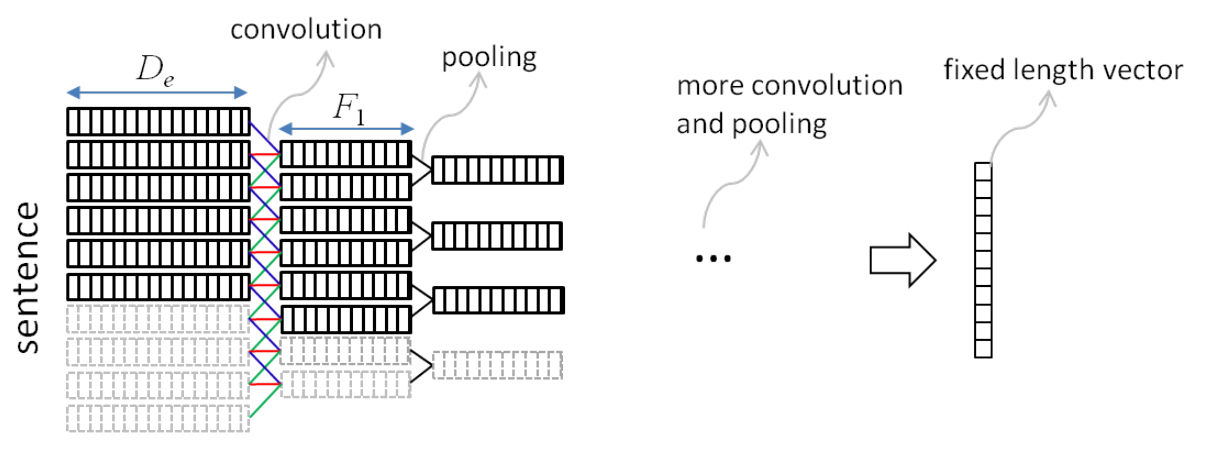
\includegraphics[width=0.9\textwidth]{arcI_arch.png}
  \caption{Architecture of arc-I}
  \label{fig:arcI_arch}
\end{figure}

\subsection{Analysis of the model}

The convolutional unit, when combined with max-pooling, can act as
the compositional operator with local selection mechanism.

The figure \ref{fig:arcI_conv} gives an example on what could happen on the first
two layers with input sentence ``the cat sat on the mat''.

3 different feature maps were chosen such that disjoint pieces of sentence were
selected (e.g. group 3 selects ``the cat'' and ``sat on'').

Different feature maps offer a variety of compositions. The pooling then
chooses, for each composition type, between two adjacent sliding windows, e.g.,
between ``on the'' and ``the mat'' for feature maps group 2 from the rightmost
two sliding windows.

\begin{figure}[H]
  \centering
  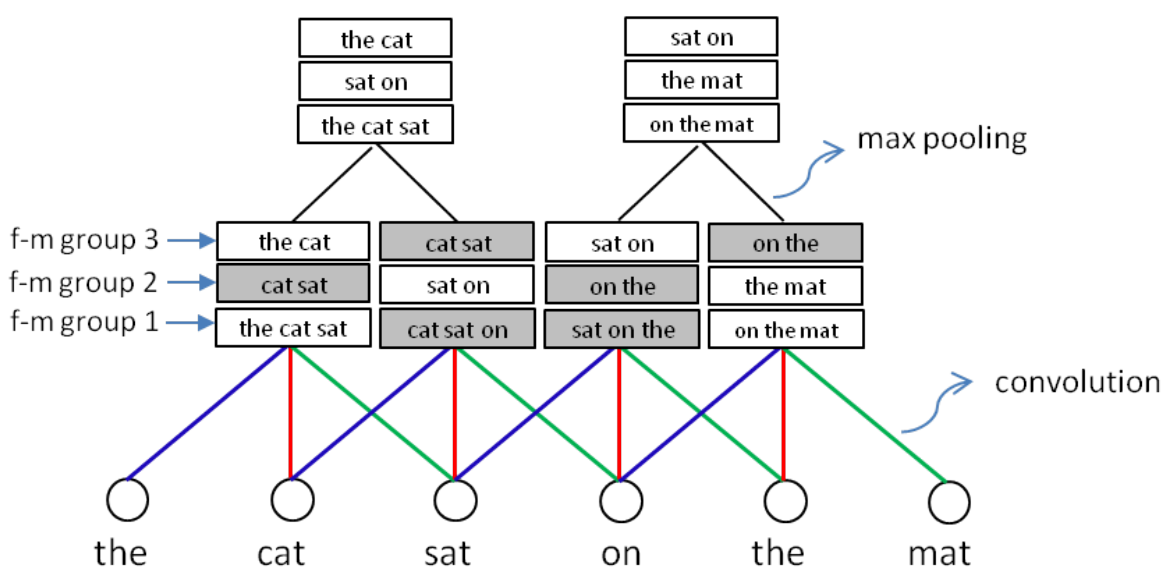
\includegraphics[width=0.9\textwidth]{arcI_conv.png}
  \caption{Analysis of arc-I}
  \label{fig:arcI_conv}
\end{figure}

\section{ARC II}

ARC II has the desirable property of letting two sentences ($S_x$ and $S_y$)
meet before their own high-level representations mature.

The Layer 0 concatenates \textit{all possible segments} of $S_x$ and $S_y$. 


The first layer applies a 1D convolution on $z^0$ and combine it with a zero gate and a sigmoid function:

\begin{equation}
\tag{First layer of ARCII, 1D convolution on two sentences segments}
z_{(i,j)}^{(1,f)} (x,y) = g(z_{(i,j)}^0) \cdot \sigma (w^{(1, f)} \cdot z_{(i,j)}^0 * b^{(1,f)})
\end{equation}

The second layer performs a 2D max-pooling in non-overlapping 2x2 windows from the 1D activation map resulting from the first layer.

The third layer performs a 2D convolution similarly to the first layer:

\begin{equation}
\tag{Thirs layer of ARCII, 2D convolution}
z_{(i,j)}^{(3,f)} (x,y) = g(z_{(i,j)}^2) \cdot \ \sigma (W^{(3, f)} \cdot z_{(i,j)}^2 * b^{(3,f)})
\end{equation}

This architecture (see \ref{fig:arcII_arch}) allows the selection not only among compositions on different segments but also among different local matchings.

ARC-II aim is to blend two seemingly diverging processes:

1) the successive composition within each sentence and
2) the extraction and fusion of matching patterns between them

\begin{figure}[H]
  \centering
  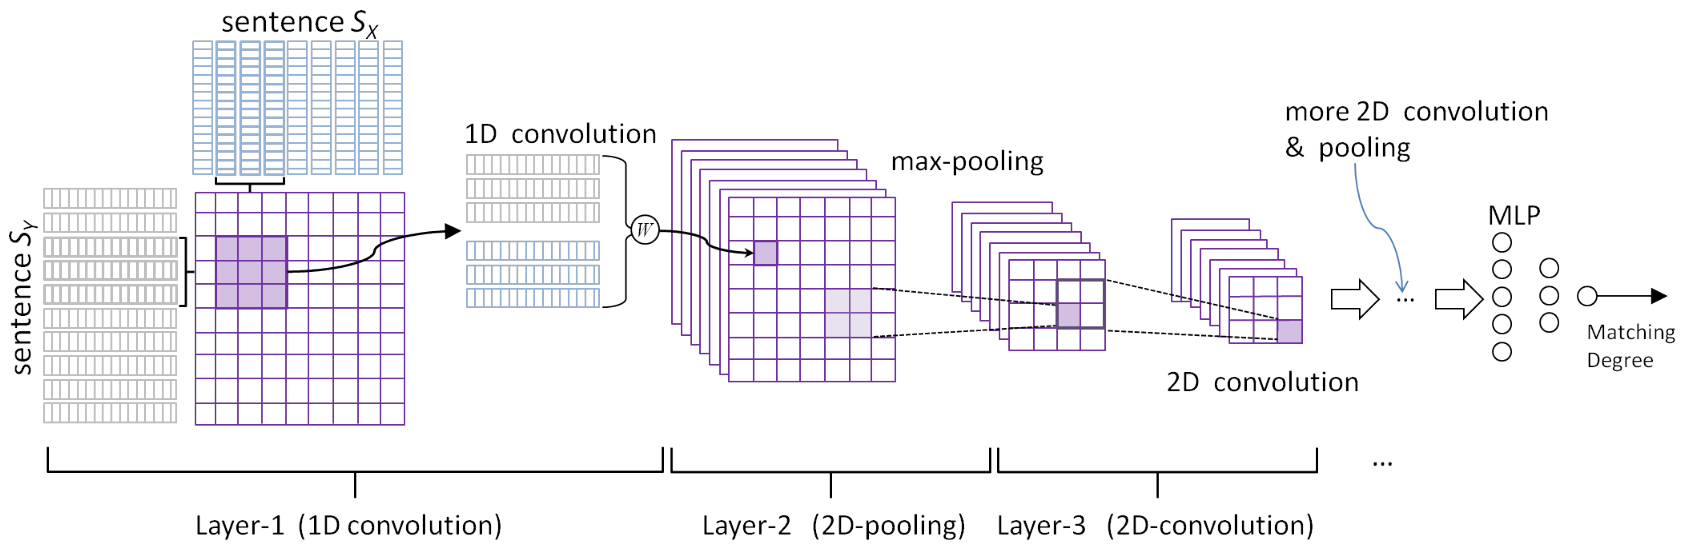
\includegraphics[width=0.9\textwidth]{arcII_arch.png}
  \caption{Architecture of arc-II}
  \label{fig:arcII_arch}
\end{figure}

\subsection{ArcII training}

The following configuration was applied also to ARC-I (see section \ref{sec:arcI}).

The loss function used is the same as in DRMM model (see \ref{chap:drmm}) and
it's the \textbf{pairwise ranking hinge loss}.

The model uses stochastic gradient descent for the optimization and perform
better with mini-batch (100 $\sim$ 200 in sizes).

For regularization \textbf{early stopping} was enough for the model with medium size
and large training sets (> 500K instances).

For small datasets (< 10k training instances) however, early stopping had to
be combined with dropout to deal with the serious overfitting problem.

\textbf{3-word window} was used throughout all experiments, but test various numbers of
\textbf{feature maps (typically from 200 to 500)}, for optimal performance.

ARC-I used two layers for convolution, two layers for pooling, and two layers
for MLP.

ARC-II used three layers for convolution, three layers for pooling, and two layers
for MLP.

\textbf{ReLu} was used as the activation function which yield comparable or better
results to sigmoid-like functions, but converges faster.
